\section{Brain}

Our robot is ultimately controled by a algorithm cuddly called the Brain.
This program is a state machine and guides the robots actions according to the state the robot is in.
The origin of the name is simple: since its job is to control everything, it must have access directly or indirectly to almost every information about the environment, like walls, obstacles, etc, and about itself, like IR sensors, odometry, etc.
This program is the only one implemented in Python instead of C++, as to make use of a software package from the ROS distribution called SMACH.
This software has the advantage of being integrated with ROS. 
We had different iterations of states, depending on which milestone we were working on specifically.
In the first iteration, we had the states: go forward, obstacle detected, turning, object detected and recognizing.

% need to insert image? it's super easier to explain (i could find it in the wiki, i thouth it was there)
The general architecture of the first iteration of the brain is presented in figure \ref{fig:1st_architecture}

\begin{figure}
\centering
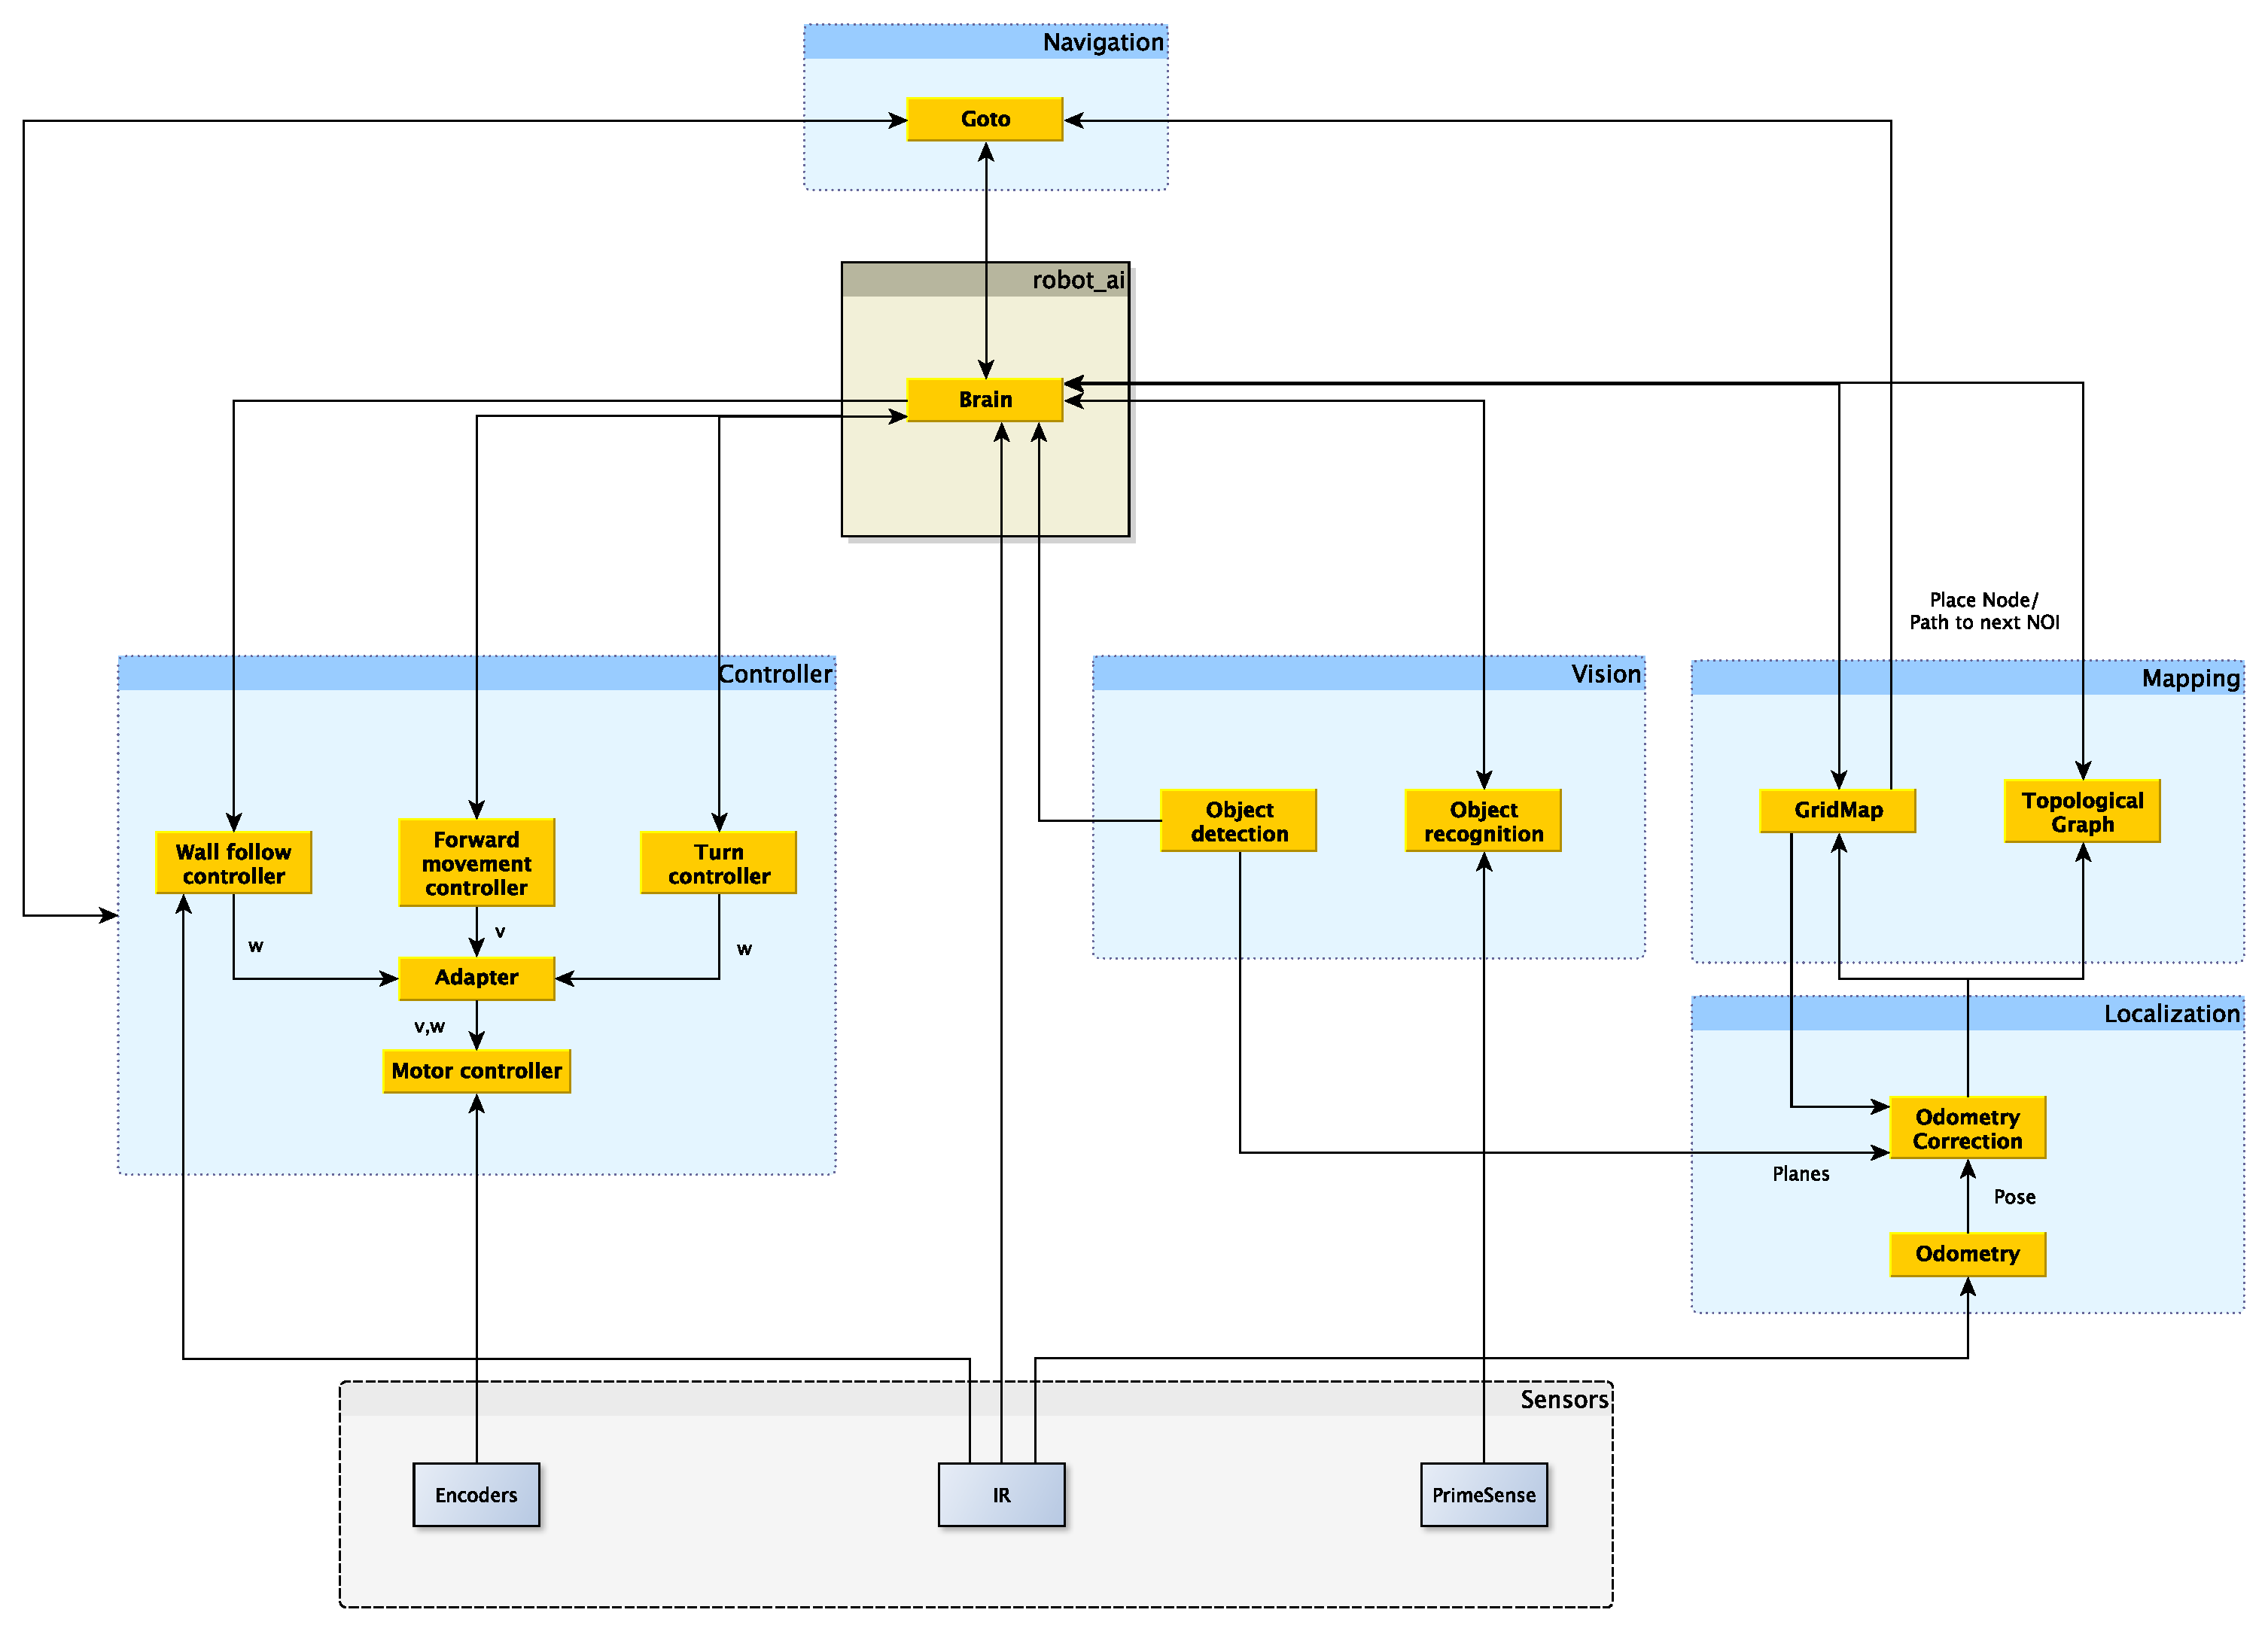
\includegraphics[width=1.0\textwidth]{figures/architecture_full.pdf}
% maybe put it elsewhere because of size?
\caption{Caption}
\label{fig:1st_architecture}
\end{figure}

With all the changes, i.e., by building on top of itself, we culminated we the states: explore, obstacle detected, object detected, follow graph and recover from crash.
Obviously the challenge is not to define the states themselves, but the conditions that lead from one state to the other.
As the project got more and more complex, so did the functions, state conditions and states themselves.
It is clear that from the first to last itaration, one main aspect that changed was the existence of a graph, explained in another section of this report, that guides the robot through the maze, when the robot is in that state, of course.

% need to insert another image? (do we have to create one or is there any picture or photo?)
